%########################################################################################
\chapter{Aflatoxin Occurrence in Kenyan Maize Fields} \label{Chapter3}
%########################################################################################

\begin{refsection} % section bibliography

\vspace*{\fill}

\large
The research in this chapter was carried out as part of the collaborative AflaZ project, entitled "Project AflaZ: Zero Aflatoxin - A Multidisciplinary Collaboration between German and African Research Institutions". This field study is a joint project of the University of Kaiserslautern-Landau (RPTU), the Kenya Agricultural and Livestock Research Organization in Kabete (KALRO Kabete), and the Max Rubner Institute in Karlsruhe (MRI Karlsruhe).

\clearpage



{\raggedright 
\
\textbf{\LARGE Analysis of aflatoxins in soils: Insights gained from a maize field study in a Kenyan hotspot region}}

%========================================================================================
\section{Introduction}
%========================================================================================

Aflatoxins are toxic secondary metabolites produced by certain fungi of the anamorphic genus \textit{Aspergillus}, which are commonly found in (sub)tropical soils where staple crops such as maize are grown \citep{mahuku2019pre}. They can enter the food chain at any stage of production by fungal infestation, from pre-harvest to post-harvest, and pose a serious health risk to humans and animals \citep{winter2019review}. In developing countries, with favorable (sub)tropical conditions for the growth and aflatoxin formation of these fungi and the limited access to control measures, outbreaks of aflatoxin contamination are common and can lead to hundreds of deaths from acute aflatoxicosis. In addition, aflatoxin contamination causes significant economic losses to the agricultural and food processing industries \citep{winter2019review}. In Kenya, maize is a essential crop that serves as both as a food and as an income source for the local population \citep{mahuku2019pre}. Unfortunately, maize is highly susceptible to infection by aflatoxigenic fungi and contamination by AFs, why AFs contaminated maize presents a severe threat to the health of Kenyan consumers who rely on maize as their staple food  with an average per capita consumption of 400 g maize per day \citep{lewis2005aflatoxin}. Furthermore, more than 75\% of maize in Kenya is produced by smallholder farmers for their own consumption, with the surplus being informally traded \citep{mahuku2019pre}. As a result, the country has witnessed multiple outbreaks of acute aflatoxicosis since 2004, leading to nearly 500 acute illnesses and 200 deaths \citep{lewis2005aflatoxin}. The economies of most tropical countries depend heavily on the export of agricultural products \citep{matumba2015concentrating}. However, importing countries, especially those in the European Union, have imposed strict legal limits on aflatoxin levels, forcing large-scale farmers to commercialize corn within the acceptable limits to these countries, while selling highly contaminated maize on the informal market or consuming it locally \citep{matumba2015concentrating, nji2022six}. As a result, the likelihood of the local population consuming contaminated food increases \citep{nji2022six, udomkun2017mycotoxins}, leading to additional economic costs such as disease costs \citep{meijer2021aflatoxin}. This situation exacerbates the health and economic problems resulting from maize contamination with aflatoxins in Kenya. Therefore, implementation of mitigation strategies to reduce aflatoxin levels in maize is critical to meet regulatory requirements, avoid crop rejection and protect consumer's health.


The most important strategy to prevent pre-harvest aflatoxin infection and resulting aflatoxin contamination is through the use of suitable soil and crop management practices \citep{fouche2020aflatoxins, verheecke2016microbial}. Different pre-harvest strategies have been proposed to reduce the incidence of aflatoxins in maize, including the use of biological control agents, crop rotation, intercropping, and less invasive soil cultivation practices. Studies have shown that the application of atoxigenic strains of \textit{A. flavus} \citep{probst2011identification} or other atoxigenic mold fungi such as \textit{Trichoderma harzianum} \citep{ren2022potential, dania2020using, sivparsad2016pre} can outcompete aflatoxigenic strains, leading to reduced growth of the toxin prducing fungi. The commercial product called "Aflasafe", based on atoxigenic \textit{Aspergillus} strains, is available in the African market and is being used for field control of aflatoxigenic fungi \citep{migwi2020assessment, bandyopadhyay2016biological}.  Intercropping, the practice of growing multiple crops together, can also reduce the occurrence of phytopathogenic fungi by disrupting the fungus's spore dispersal patterns and suppressing pest insects \citep{trenbath1993intercropping, langer2007intercropping}. Pest insects can cause physical damage to the crops and facilitate spore transport through wounds, thereby exacerbating fungal infection. Intercropping can help to alleviate this issue by creating a physical or chemical barrier \citep{trenbath1993intercropping, langer2007intercropping}. In context of maize cultivation, a "push–pull" intercropping technique  has been demonstrated to be an effective method for controlling important maize pests such as several stemborers and the fall army worm (\textit{Spodoptera frugiperda}) and reducing AFs prevalence in maize fields \citep{njeru2020impact}. This technique involves intercropping maize, with insect-repellent forage legumes from the genus \textit{Desmodium} and planting Napier grass (\textit{Pennisetum purpureum}) around the field. The \textit{Desmodium} legume releases semiochemicals that repel stemborer moths ("push") while simultaneously attracting them to the Napier grass ("pull"), which release attractive volatile organic compounds \citep{njeru2020impact, khan2000exploiting, khan2011push}. However, the Napier grass does not support significant survival of emerging larvae, thereby preventing their destruction of the grass \citep{njeru2020impact, khan2011push}. The push-pull system also effectively controls the fall army worm, an invasive pest that recently invaded Africa and attacks maize and other crops \citep{njeru2020impact, khan2011push}. Conservation tillage is a practice that limits the disruption of the soil's structure, primarily through non-inversion techniques. By leaving over one-third of the soil surface covered by crop residues, conservation tillage promote and sustain soil health while preventing soil degradation \citep{peigne2007conservation}. Conservation tillage offers several benefits in organic farming, such as decreased erosion, enhanced macroporosity on the soil surface due to an increased number of earthworms, higher microbial activity, and greater carbon storage \citep{busari2015conservation}. Additionally, it lowers nutrient run-off and leaching, minimizes fuel consumption, and speeds up tillage \citep{busari2015conservation}. Consequently, by improving soil health, conservation tillage may enhance plant health and lead to greater resistance against fungal pathogens. Conversely, if crop residues contaminated with aflatoxigenic fungi are left on the field for an extended period, there is a risk of soil re-contamination and subsequent crop contamination  \citep{fouche2020aflatoxins, accinelli2008aspergillus, angle1987aflatoxin}. Since AFs are known to be toxic to certain soil microorganisms \citep{burmeister1966survey, arai1967antimicrobial}, an increase of their presence in soil may affect ecological balance of the soil microbiome and associated functions.


The effects of pre-harvest mitigation strategies have been studied mainly in terms of plant health and plant contamination by fungi and their toxins, but very little information is available on aflatoxin contamination and its toxicological consequences for the soil ecosystem. These strategies are reported to alter "aboveground" aflatoxin occurrence, but the consequences for "belowground" aflatoxin occurrence are literarily unknown. Consequently, the aim of the present study was to investigate  whether the agricultural practices change the concentration of AFs in field soil. These practices included push-pull intercropping, application of a suspension of \textit{Trichoderma harzianum}, conservation tillage, and a control that followed conventional farming practices, as typically practiced by local small scale farmers. In the context of conservation tillage, contaminated residues may remain on the soil surface, potentially acting as a source of AFs. Therefore, we hypothesized elevated AFs levels in fields with conservation tillage and in particular at the top-soil layer. Furthermore, since the microbial and physico-chemical soil conditions in root space and inter-plant zone differ, I assume that there are differences in the production and transformation processes of AFs, which is reflected in differences in the levels of AFs. The farming practices "Trichoderma" and "push-pull" which have been reported to decrease the presence of aflatoxigenic fungi, enhance the crop plants’ resistance to fungal infestation and reduce aflatoxin prevalence in crops. Therefore I, hypothesize reduced AF levels in soils managed with these practices compared to those managed conventionally.

%========================================================================================
\section{Material and Methods}
%========================================================================================

%----------------------------------------------------------------------------------------
\subsection{Study Design and Field Treatments}
%----------------------------------------------------------------------------------------

The field study was conducted within the framework of the AflaZ project. The AflaZ project (Project AflaZ: Zero Aflatoxin) is an international and multidisciplinary research collaboration between German and African research institutions, aimed at reducing aflatoxin contamination in maize and milk in Kenya. The project focus on the development of strategies to reduce the formation of aflatoxin by investigating the overall context of the problem, including plant protection, soil health, insect control, and molecular biological analyses, as well as knowledge transfer, networking and capacity building. 

%++++++++++++++++++++++++++++++++++++++++++++++++++++++++++++++++++++++++++++++++++++++++
\begin{figure}[b!]
\centering
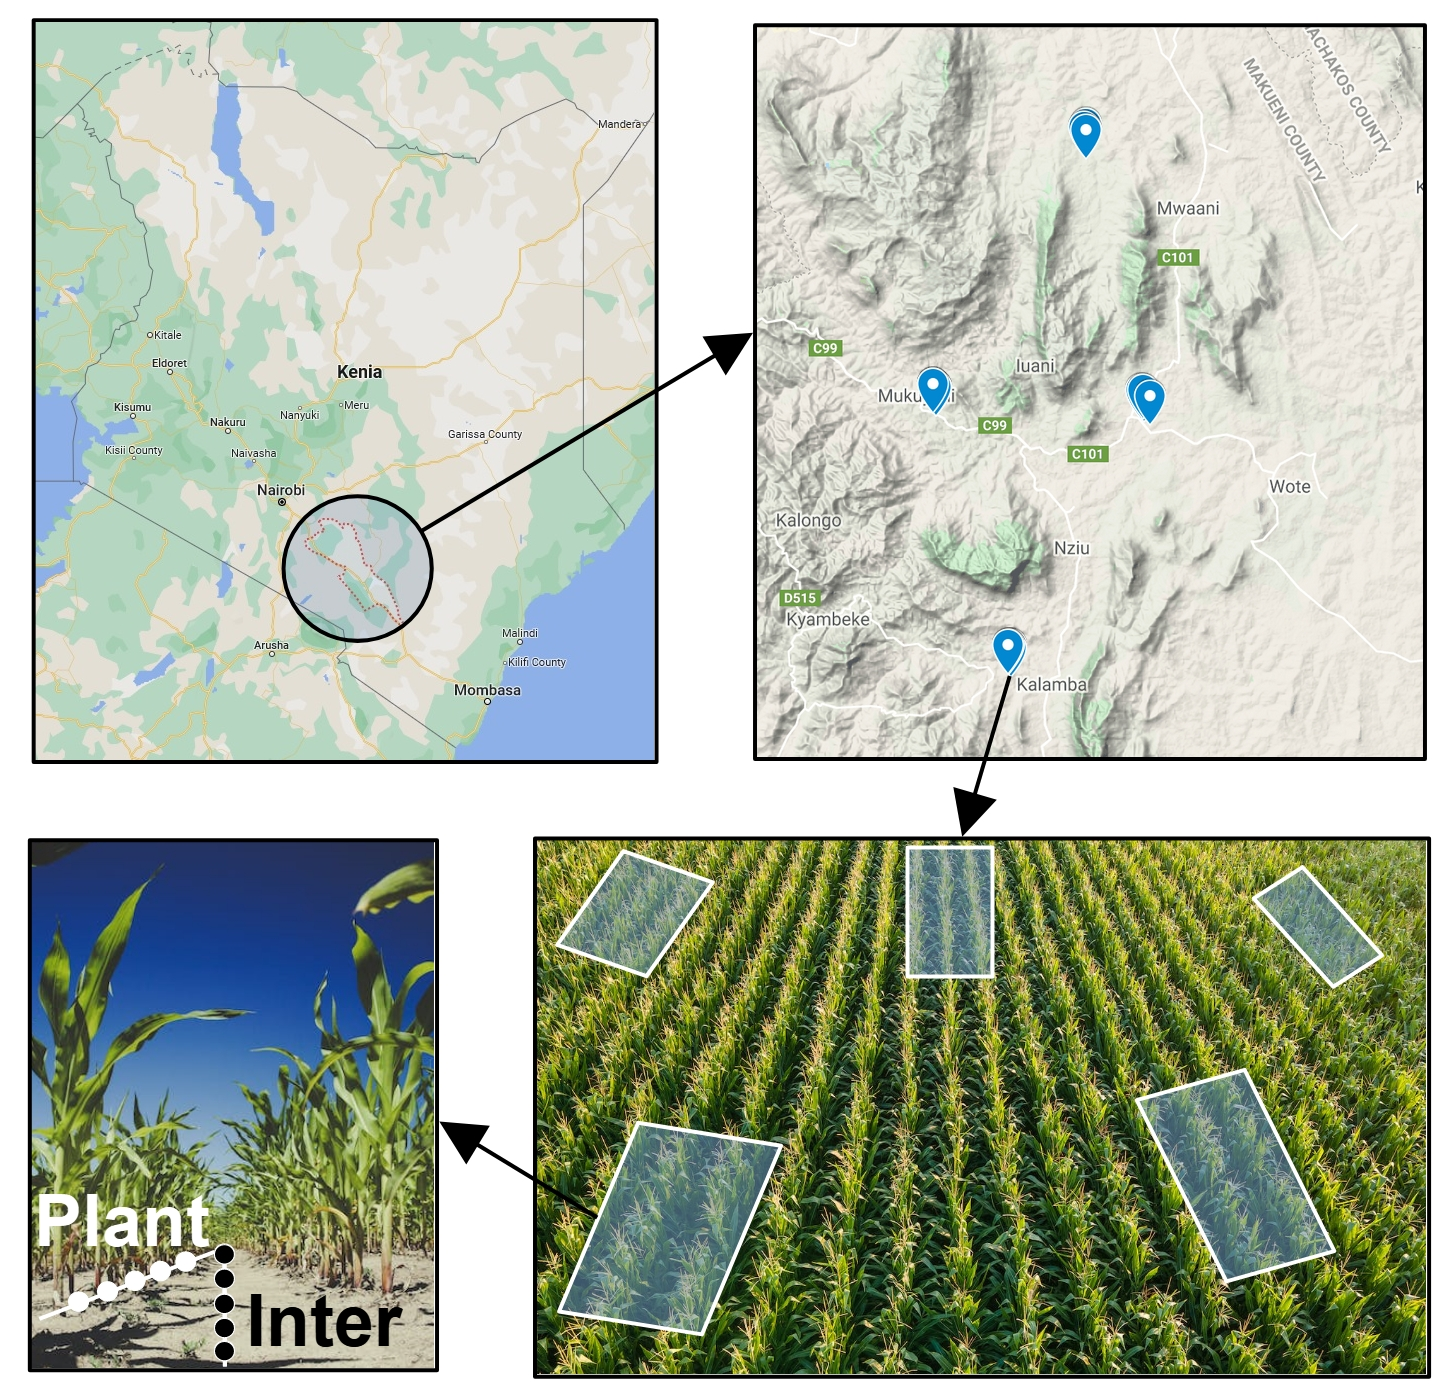
\includegraphics[width=1\textwidth]{figures/kenya field sampling.jpg}
\decoRule
\captionsetup{labelfont=bf, justification=justified, singlelinecheck=false, width=1\textwidth}
\caption{Study sites and sampling scheme for maize fields in the Makueni region (highlighted in top left map). 16 fields were selected within the Makueni county (markings in top right map). Five clusters were designated on each field (bottom right). Each cluster was sampled on two positions at-"Plant" and "Inter"-row (represented by white and black dots, respectively) and two depths (top- and subsoil). Map data: ©2022 Google, Sanborn, USA.}
\label{fig:Kenya_sampling}
\end{figure}
%++++++++++++++++++++++++++++++++++++++++++++++++++++++++++++++++++++++++++++++++++++++++


As part of the AflaZ project, a field study was carried out in a high-risk model region for aflatoxin contamination in Sub-Saharan Africa, namely maize fields in the Makueni region. The Makueni region was purposely selected based on previously reported outbreaks aflatoxicosis \citep{lewis2005aflatoxin}. The field experiments and sample collections were organized and executed by the Kenya Agricultural and Livestock Research Organization (KALRO), while local farmers carried out the maize planting according to the instruction provided by the institution. Over the course of three consecutive growing seasons, the effect of treatments on fungal and aflatoxin contamination in soil and maize grain was examined. The study involved 12 farmers from each of three villages in Makueni County: Ukia, Kisau-Kiteta, and Nzaui-Kilili-Kalamba. Two different types of crops were used, DK 8031 maize and KAT B1 beans, as well as Duma 43 and KAT B1 beans during the long and short rain season. Maize was planted at a spacing of 75cm x 30cm with two seeds per hill and a row of beans spaced at 4cm between the maize rows. Conservational tillage was applied by spraying with Gramoxone® (25.4\% active ingredient Paraquat, Syngenta, Basel, Switzerland) at the recommended field application rate after planting the maize and legumes, but before the two crops had germinated. For the remaining three treatments, hand weeding was done after planting maize intercropped with beans or desmodium depending on the plots. A total of 16 fields from 4 regional clusters, each farmed with one of the respective treatments, were sampled (see Figure \ref{fig:Kenya_sampling}).

%----------------------------------------------------------------------------------------
\subsection{Soil Sampling Procedure}
%----------------------------------------------------------------------------------------

During the third season of maize cultivation in August 2020, soil sampling was conducted for the present study. Following a Standard Operating Procedure (SOP) developed at the University of Kaiserslautern--Landau (RPTU), the sampling was conducted with the support of KALRO (SOP available in Chapter \ref{Annex_chap3}). Five sub-plots of approximately 500 m\textsuperscript{2} were defined on each field, with sampling points evenly distributed within each sub-plot. Soil samples were collected at two depths (0-15 and 15-30 cm) and two positions (between plants and inter-row) to detect potential concentration differences. Ten samples were taken for each position-depth combination, resulting in 10 individual samples per sub-plot. Sampling was conducted by pushing an augur vertically into the soil to a depth of approximately 35-40 cm and separating the soil core into topsoil and subsoil fractions. Individual samples were pooled to create one sample for each position-depth combination within a sub-plot. The sampling design is visualized in Figure \ref{fig:Kenya_sampling}. Sampling was completed by August 31st, 2020, and the samples were stored at 4°C in the dark until shipment. Soil samples were shipped to Germany on September 16th, 2020 for aflatoxin analyses. Upon arrival in Germany on November 16th, 2020, the samples were immediately quarantined at room temperature for 3 weeks. Subsequently, they were stored at -20°C until further processing.


%----------------------------------------------------------------------------------------
\subsection{Aflatoxin Analysis}
%----------------------------------------------------------------------------------------

Soil samples were passed through a 2 mm stainless steel sieve and analyzed for AFB1, AFB2, AFG1 and AFG2 according to \citet{albert2021validation}. Briefly, soil samples were extracted with MeCN:\ce{H2O} at a soil:solvent ratio of 1 g : 3 mL by orbital shaking and ultrasonication treatment and analyzed via both, high performance liquid chromatography with mass spectrometry (LC-MS) and fluorescence detection (HPLC-FLD). The presence of interference peaks and matrix effects was tested by comparing a matrix-matched and solvent calibration \citep{albert2021validation}. A matrix blank solution was prepared by combining equal volumes of all extracted samples.

%========================================================================================
\section{Results and Discussion}
%========================================================================================

\subsection{Absence of aflatoxins in the soil samples}
No aflatoxins were detected in any of the 320 soil samples. The chromatograms of both HPLC-FLD and LC-MS showed no interferences in the time window of the respective aflatoxins in both, the samples and the matrix blank solution.
As a result, the initial research question concerning the influence of farming practices on the presence of aflatoxins in field soils remained unresolved. Nevertheless, this outcome has raised supplementary questions regarding the absence of aflatoxins in the examined soils.  There are several possible explanations for the non-detectability of aflatoxins: (1) absence of any aflatoxigenic fungal strain in the fields studied; (2) Insufficient sampling strategy to detect aflatoxins in the soil; (3) (Photo)chemical and microbial degradation of aflatoxins in the field and/or during sample transport to Germany. These potential causes will be evaluated for their plausibility in the subsequent sections.

%----------------------------------------------------------------------------------------
\subsection{Aflatoxigenic Strains in the Field Soil}
%----------------------------------------------------------------------------------------

It is reported that there are temporal dynamics, both within and between years, regarding the occurrence of toxigenic fungal strains and mycotoxins in crop plants and debris \citep{abbas2008dynamics, orum1997spatial, ching2022spatial}. These dynamics can be due to various reasons such as climatic conditions, previous agricultural practices and the stage of development of the crop \citep{ching2022spatial, dutta2001isolation, jaime2010crop}. It is therefore conceivable that the field sampling fell into a time window with low occurrence of toxigenic strains and/or reduced aflatoxin production. However, this is contradicted by the fact that toxigenic strains were found in the same soil samples by another team of researchers from the MRI (presented at the AflaZ congress on October 13th, 2022 in Nairobi, Kenya). The ability of fungal strains of \textit{A. minisclerotigenes} and \textit{A. flavus} isolated from soils, to produce AFs was confirmed through the detection of AFs in extracts from cultivated fungal strains using thin-layer chromatography with fluorescence detection. Additionally, findings presented by the KARLO-Kabete Institute at the AflaZ congress on October 13th, 2022 (Nairobi, Kenya),  indicated the presence of toxigenic strains in the fields, as demonstrated by the detection of AFs in grain samples. Overall, the absence of aflatoxigenic strains in the fields seems rather implausible as an explanation for the non-detectability of AFs in the soil samples.

%----------------------------------------------------------------------------------------
\subsection{Sampling Strategy to Detect Aflatoxins in the Soil}
%----------------------------------------------------------------------------------------

Agricultural soils exhibit inherent heterogeneity, both spatially across the field and vertically within the soil profile, leading to potential variations in mycotoxin levels even within a small area. Certain plant debris, particularly grain-rich material, is often heavily colonized by toxigenic \textit{Aspergillus} fungi, making them potential "hot spots" for aflatoxin contamination, with concentrations reaching up to 10\textsuperscript{2} \textmu g kg\textsuperscript{-1} \citep{accinelli2008aspergillus}. Therefore, one possible explanation for the absence of detectable AFs in soil samples could be an inadequate sampling procedure that failed to capture these localized "hot spot" areas within the soil. However, this assumption is contradicted by the successful application of the same sampling strategy in maize field soils in Germany to detect Fusarium toxins including nivalenol and deoxynivalenol (DON) \citep{kenngott2022fusarium}. Therefore, this explanation also appears implausible,  particularly considering that soil extracts from the Kenyan soils were also subjected to the same analytical procedure described by \citet{kenngott2022fusarium} and tested negative for the presence of Fusarium toxins, including nivalenol, deoxynivalenol, 15-acetyl-deoxynivalenol, and zearalenone.

%----------------------------------------------------------------------------------------
\subsection{Aflatoxin Degradation}
%----------------------------------------------------------------------------------------

Soil sampling was conducted during harvest season, which fell into the dry season with low moisture and high temperature conditions. Farmers leave the maize plants in the field for several weeks during this period in order to decrease the moisture content of the kernels before harvesting. This initial drying in the field effectively reduces moisture content and prepares the crop for the subsequent drying processes required for storage and sale. The plants undergo senescence, and the leaves begin to wilt, consequently reducing leaf coverage and allowing more sunlight to reach the ground. As a result, aflatoxin-contaminated material on the soil surface and in the topsoil layer could be exposed to UV light. It is well established that AFs are highly susceptible to photolytic degradation, with a half-life ranging from a few hours to days under direct irradiation \citep{diao2015ultraviolet}. This suggests that photolytic degradation of aflatoxins may have occurred in the field shortly before sampling, which could explain the absence of aflatoxins in the collected samples. 

In addition, a period of 2.5 months passed between sample collection and their arrival in Germany. While the samples were kept refrigerated at 4°C until being shipped, they were not refrigerated during the 2-month transport period. This extended duration may have led to degradation of AFs. Furthermore, the samples were subjected to extremely dry conditions during the dry season, characterized by a lack of rainfall and high temperatures, which would have resulted in significantly reduced microbial activity. However, it is also possible that abiotic degradation occurred in the absence of light. It is important to note that the prevailing consensus is that abiotic degradation of aflatoxins does not play a major role in the soil environment. However, the experimental evidence is very limited- In this regard, only two studies have conducted degradation experiments under (near) sterile conditions, and their findings indicated minimal degradation of AFB1 \citep{accinelli2008aspergillus, starr2017solvent}. Considering these factors, the likelihood of abiotic degradation during transport appears less plausible.


Microbial degradation is widely recognized as a significant process contributing to the removal of aflatoxins in soil \citep{fouche2020aflatoxins}. Previous studies have reported almost complete dissipation of AFB1 at concentrations ranging from 10\textsuperscript{0} to 10\textsuperscript{4} \textmu g kg\textsuperscript{-1}  within a week in soil \citep{angle1980decomposition, angle1986aflatoxin, accinelli2008aspergillus}. However, considering the arid conditions prevailing during the harvest season in the field, it is expected that microbial activity will be severely limited. Additionally, the low moisture content observed in the soil samples suggests that microbial degradation during shipment is unlikely. During the transitional phase between seed ripening and senescence, nutrient, moisture and temperature conditions are heavily changing towards unfavorable conditions i.e. drought, heat and reduced root exsudation \citep{zhalnina2018dynamic, cotta2013temporal}. However, large amounts of carbon and nitrogen are released by dead roots and it was shown that  soils can be hotspot of microbial activity at this stage \citep{spohn2014spatial}. Thus, during this phase, any existing AFs in the soil could still potentially undergo microbial degradation. Consequently, microbial degradation during the transition to the senescence phase could have contributed to a reduction in soil contamination before and at early stages of the harvest season, even if minimal aflatoxin degradation is expected during later stages of the harvest season with very dry soil conditions.

%========================================================================================
\section{Conclusion and Future Perspectives}
%========================================================================================

Suitable soil and crop management practices are considered the major means of preventing pre-harvest aflatoxigenic fungal infestation and aflatoxin contamination and thus ensure soil health and productivity. The present study was therefore designed to investigate how different farming practices affect the occurrence and distribution of aflatoxins in the soils of maize fields. However, the research question could not be addressed due to the absence of aflatoxins in any of the soil samples. The absence of AFs in the soil during the whole period of maize cultivation seems unlikely in view of the proven presence of toxigenic strains in the samples. Since the mycotoxin producing fungi were identified in the soil samples, this may have the potential of a production \textit{in situ} in early stages of plant growing (i.e. when soil moisture recovers) with the risk of a translocation from soil to plant. Moreover, methodological shortcomings in the sampling strategy seem improbable, as previous studies have detected mycotoxins in maize field soils using the same sampling strategy. Rather, a (photo)chemical or microbial degradation of the aflatoxins up to non-detectability in the field, during sample storage or the extended period of sample transport may have occurred. To gain a comprehensive understanding of the persistence and environmental behavior of AFs in soil, we recommend conducting microcosm experiments under controlled conditions to evaluate the likelihood, significance, and mechanisms of the various degradation processes. Furthermore, for future studies on the impact of farming practices on pre-harvest soil contamination with aflatoxins, we propose a temporally close-meshed sampling over the entire course of maize cultivation period to understand the temporal dynamics in aflatoxin occurrence. In addition, we emphasize the importance of conducting prompt analyses of soil samples subsequent to sampling to minimize potential degradation during transportation and storage, highlighting the necessity for capacity building and close collaboration with local analytical partners to establish analytical capabilities in close proximity to the fields.

%========================================================================================
\section{References}
%========================================================================================

\printbibliography[segment=\therefsegment, heading=none]

\end{refsection}
